\section{Implementing Synchronization}\label{sec:impl_sync}
In this section we discuss how we implement the methods of synchronization we discussed in \cref{cha:sync}.
First we summarize what lead us to implementing synchronization the way we did.
Then we will explain how each of the implemented synchronization methods work, and lastly we explain where we use the synchronization in the app.

In it we decided, in \cref{sec:sync_conclusion}, that NTP would suit us best.
However for practical reason we decided to implement \ac{SNTP}, which as the name suggests is a simplified version of \ac{NTP}, but does not require storing the state over time.
This solution requires each device to synchronize with an \ac{NTP}-server over the internet.

Since a persistent internet connection is not an ideal requirement for our application we also implemented our own time-synchronization over the local network, we create using WiFi Direct.
This method would not synchronize each client to a global clock, like \ac{NTP} and \ac{SNTP} does, but rather synchronize the clock of the clients to the clock of the server.
However for our application this it not a worry, our goal is to synchronize audio accurately across devices in our network, which does not require each clock to be globally synchronized, only locally.

We decided to implement both of these, that is \ac{SNTP} over the internet and time-synchronization over the WiFi Direct.
Then we will benchmark them to determine the solution which requires internet is better, and thusly justify the added requirement for the users.

As a side note, it is not possible for non-rooted Android devices to change the clock of the device, except with manual input in the setting menu.
For this reason we will not synchronize our clocks on the devices, but rather find the offset between the clock on a given device, and the clock of the \ac{NTP}-server or master.

\subsection{\ac{SNTP} over the Internet}
In this method, the goal is to get the offset of every device in the network, clients and server, relative to a 3rd party \ac{NTP}-server.


\begin{figure}[htb]
    \centering
    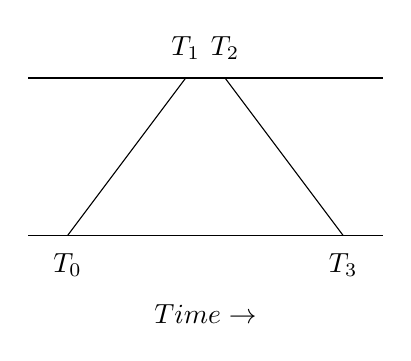
\begin{tikzpicture}[auto]
        \draw (0, 0) -- (4.5, 0);
        \draw (0,-2) -- (4.5,-2);

        \draw (0.5, -2) -- (2, 0);
        \draw (4.0, -2) -- (2.5, 0);

        \draw (2.25, -3) node {$Time \rightarrow$} node[above=3pt] {$   $};

        \draw (0.5, -2) node[below=3pt] {$T_0$};
        \draw (4.0, -2) node[below=3pt] {$T_3$};
        \draw (2  ,  0) node[above=3pt] {$T_1$};
        \draw (2.5,  0) node[above=3pt] {$T_2$};
    \end{tikzpicture}
    \caption{Caption here}
    \label{fig:ntp_packets}
\end{figure}

\subsection{Time-synchronization over WiFi Direct}

\subsection{Using the Synchronization in the App}
For simplicity we decided to use the offset our synchronization gave us just before sending messages over the network, and just after receiving them.
That is, when we send a message, the timestamp in it is of the master clock, and when we receive a message, it is converted to the local clock.

This has some advantages and disadvantages, the biggest advantage is simplicity, it allows us to only think about time synchronization in one place, and not in the player itself.
However the disadvantage is that the longer we buffer data, the more outdated it gets.
